% Appendix (optional)
% Add supplementary material here if needed.

\section*{Appendix}

\subsection*{A. Additional Figures}

\begin{figure}[h]
\centering
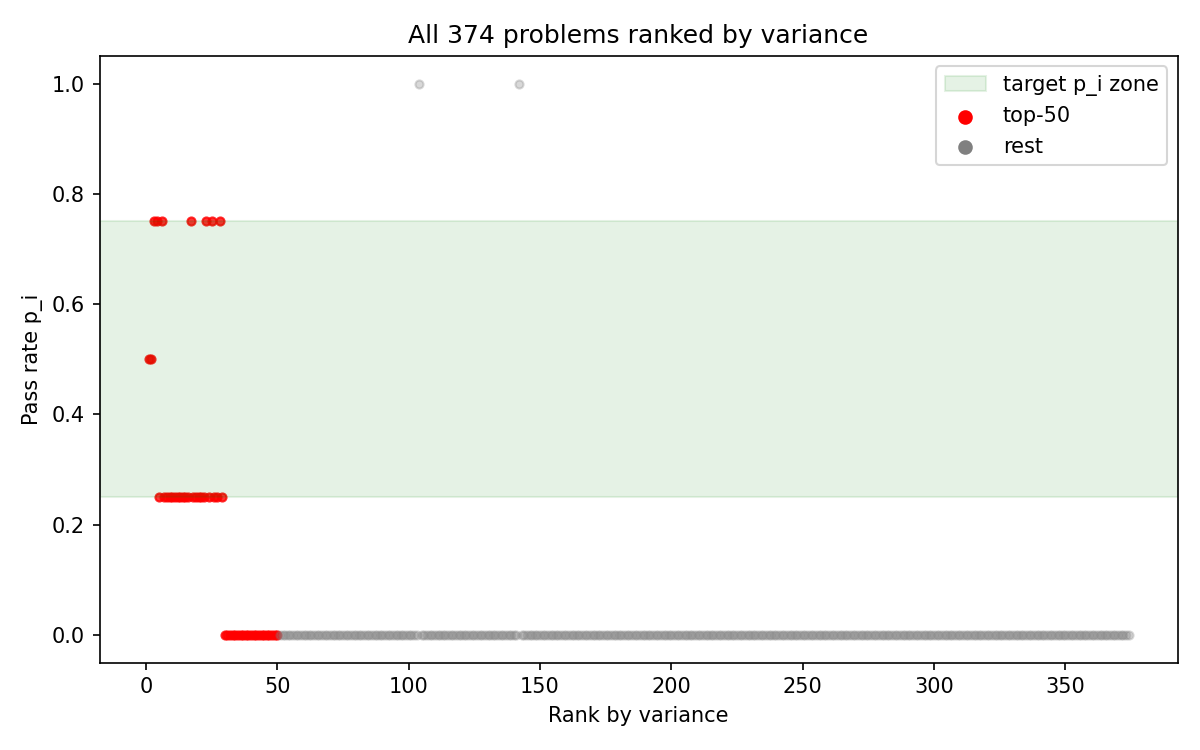
\includegraphics[width=0.9\textwidth]{figures/fig4_top_scatter.png}
\caption{Scatter plot of per-problem variance scores for the top-50 variance-selected problems. The 29 high-variance problems ($v_i=0.1875$) cluster at the top, with 21 zero-variance filler problems included due to the boundary gap (\texttt{boundary\_gap=0}).}
\label{fig:top_scatter}
\end{figure}

\begin{figure}[h]
\centering
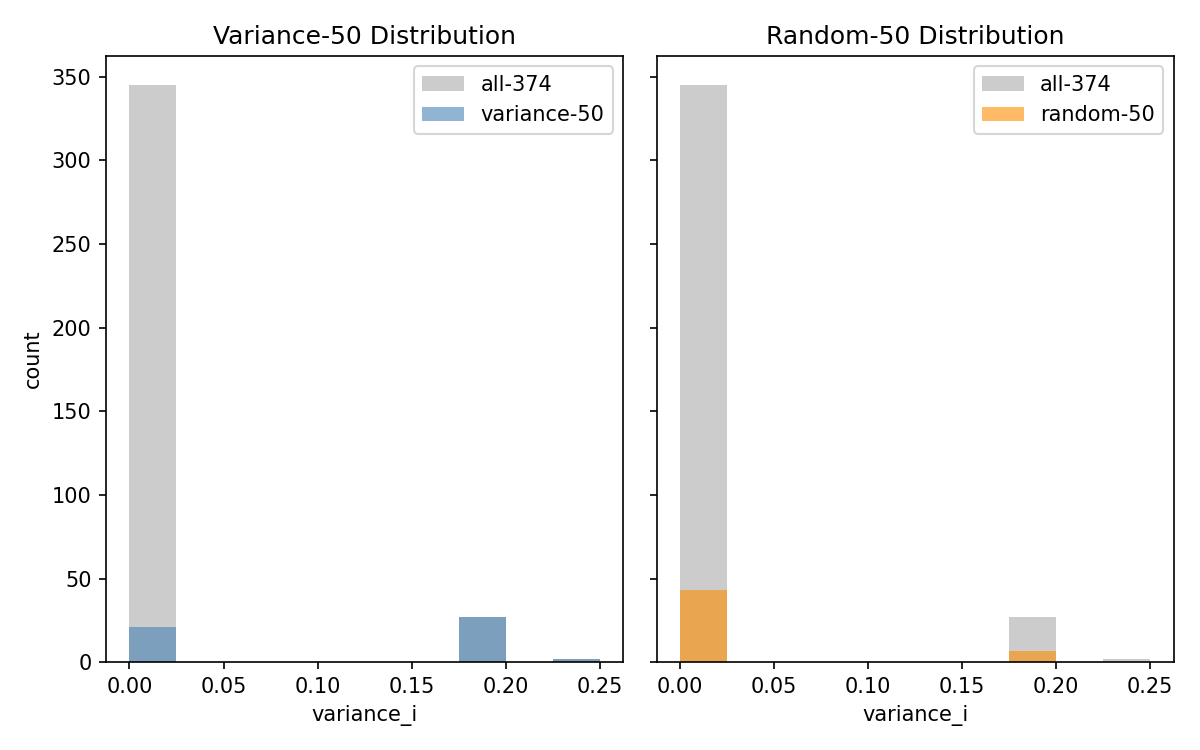
\includegraphics[width=0.9\textwidth]{figures/fig2_histograms.png}
\caption{Variance distribution comparison between variance-50 and random-50 selections. The variance-guided selection concentrates mass at $v_i=0.1875$, while random selection predominantly draws from the zero-variance pool.}
\label{fig:histograms}
\end{figure}

\begin{figure}[h]
\centering
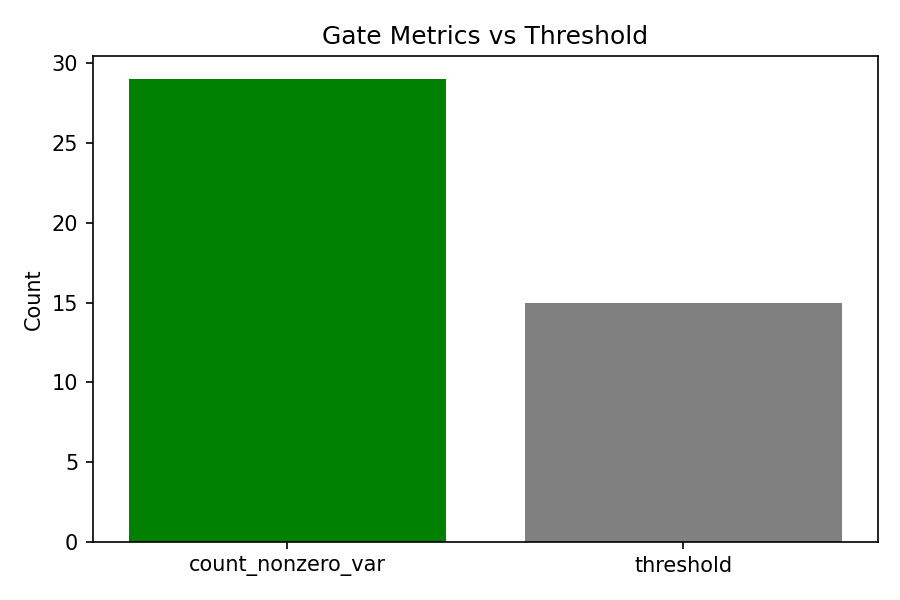
\includegraphics[width=0.7\textwidth]{figures/fig1_gate_metrics.png}
\caption{Gate metric summary for h-e1: count of problems with nonzero variance against the threshold of 15. 29 problems exceed threshold (PASSED).}
\label{fig:gate_metrics}
\end{figure}
